\documentclass[letterpaper,10pt,twocolumn,titlepage]{article}

\usepackage{graphicx}                                        
\usepackage{amssymb}                                         
\usepackage{amsmath}                                         
\usepackage{amsthm}                                          

\usepackage{alltt}                                           
\usepackage{float}
\usepackage{color}
\usepackage{url}

\usepackage{balance}
\usepackage[TABBOTCAP, tight]{subfigure}
\usepackage{enumitem}
\usepackage{pstricks, pst-node}


\usepackage{geometry}
\geometry{textheight=8.5in, textwidth=7in}

%random comment

\newcommand{\cred}[1]{{\color{red}#1}}
\newcommand{\cblue}[1]{{\color{blue}#1}}

\usepackage{hyperref}
\usepackage{geometry}

\def\name{Savannah Van Beek}


%% The following metadata will show up in the PDF properties
\hypersetup{
  colorlinks = true,
  urlcolor = black,
  pdfauthor = {\name},
  pdfkeywords = {cs311 ``operating systems'' files filesystem I/O},
  pdftitle = {CS 311 Project 2: UNIX File I/O},
  pdfsubject = {CS 311 Project 2},
  pdfpagemode = UseNone
}

\begin{document}
Savannah Van Beek \newline
CS 311			  \newline
02-08-2012		  \newline

\begin{figure}[h!]
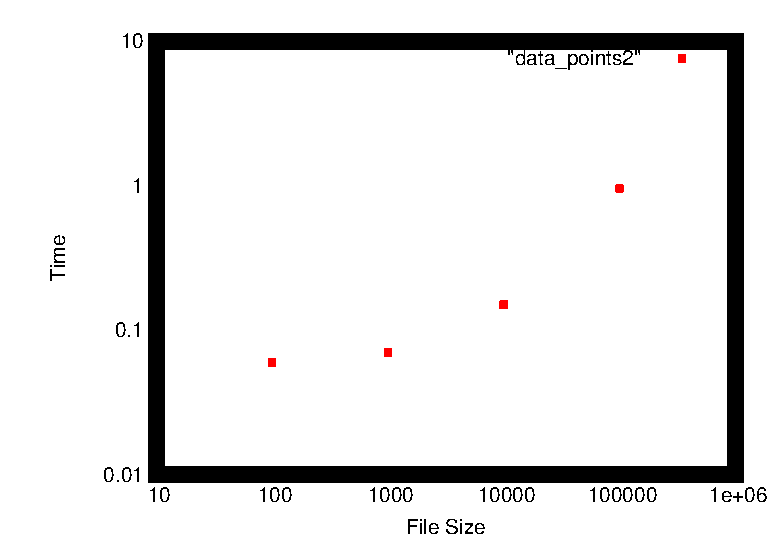
\includegraphics[width=6in, height=3in]{things.eps}
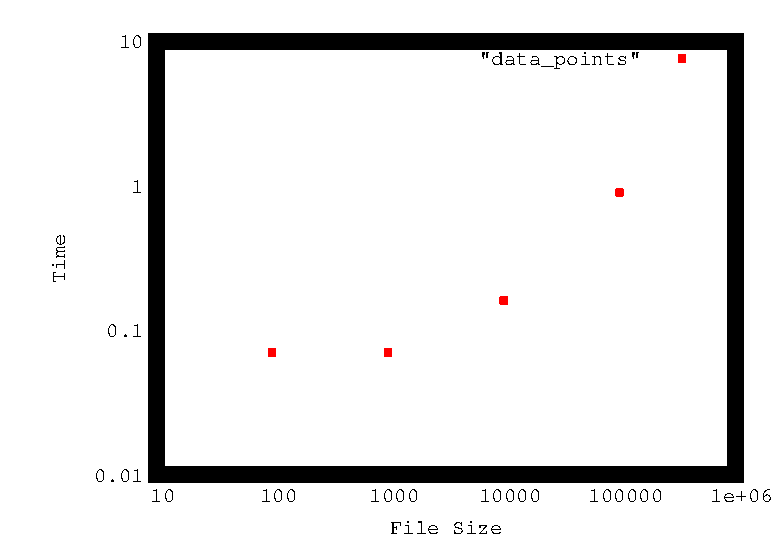
\includegraphics[width=6in, height=3in]{stuff.eps}

\end{figure}

My design decisions for this assignment consisted of not using malloc, hard coding the number of children (for a total of 50), not reading in input from the user for the number of children, left punctuation in, and I didn't use functions. I was originally planning on going back and use mallac since I didn't with the last assignment, but I ran out of time trying to just get the program working to go back and try to implement malloc. So because of that I just hard coded the number of children that the 
\vfill\break
\vspace*{6.82in}
program makes at 50. Then when parsing I chose to leave the punctuation in including periods, comas, and apostrophes. I also chose not to use functions. Not for any real reason, I just ended up putting it all in the one file. I also recieved debugging help from Jonah Brooks.

\vfill\break

\begin{tabular}{ | p{3in} | p{3in} | } 
\hline 
Commit time & Commit Message \\ \hline
\input{glogs}
\end{tabular}
 
\end{document}
